\chapter{Results}

\section{Exploiting Android x86}

\begin{figure}[!ht]
  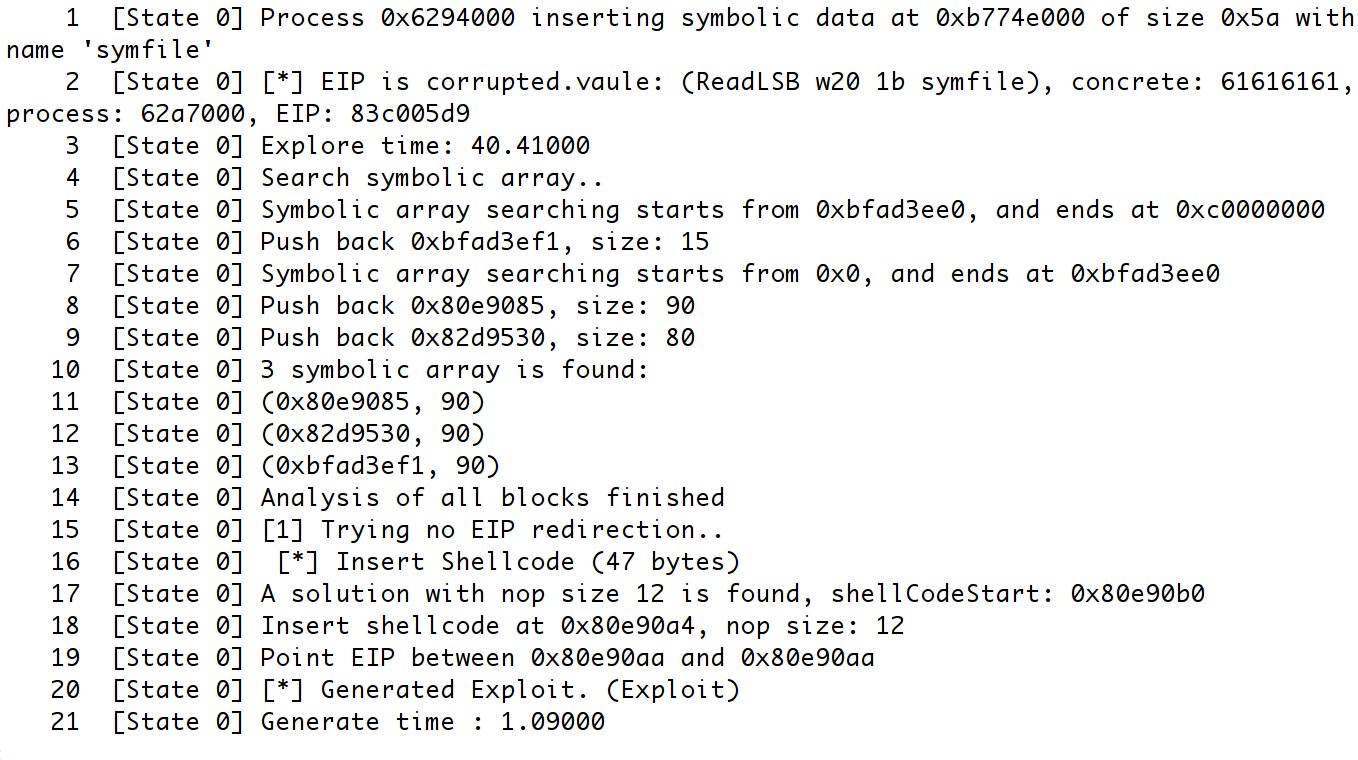
\includegraphics[width=\textwidth]{exploit-progress}
  \caption{Android x86 Exploit Progress}
  \label{fig:exploit-progress}
\end{figure}

Figure~\ref{fig:exploit-progress} shows the progress of exploit generation. A
file with 90 (0x5a) bytes of the size is mapped into memory and marked as
symbolic as shown on line 1. Starting from line 2, the message indicates that
some part of the symbolic data has tainted the eip register and thus triggers
the exploit generating process. The record shows that the eip register is
overwritten by value 0x61616161, which is the hexadecimal representation of the
string ``aaaa'', starting from the 27th byte of the overall symbolic data.
The process then searches through all memory space to collect memory chunks
that are tainted by the symbolic input. We name these chunks of memory as
symbolic array. In this example, three symbolic arrays with size 90 bytes, 80
bytes, and 15 bytes have been found. The process then tries to inject three
pieces of data into a symbolic array, a piece of pre-generated shellcode, a NOP
sled, and the address pointed to somewhere in-between the NOP sled. The process
would start to generate exploit with the largest array, and move on to the next
one if the current one does not satisfy all the constraints.

The generated exploit is shown as Figure~\ref{fig:exploit-input} in hexadecimal
format. This exploit uses a shellcode that would write the string ``Exploit!''
into Android logging service. The shellcode could be considered the same as
the following C code snippet

\inputminted[fontsize=\footnotesize]{c}{source/execve-log.c}

\begin{figure}[!ht]
  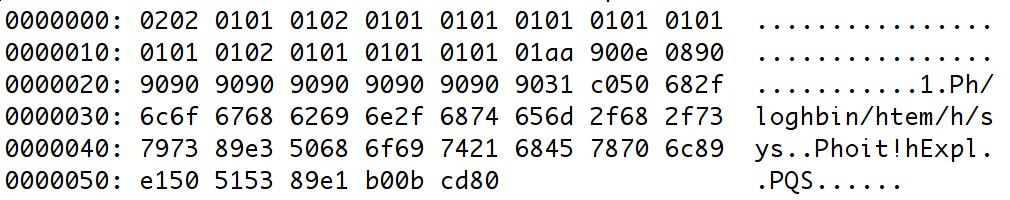
\includegraphics[width=\textwidth]{exploit-input}
  \caption{Generated Exploit Input}
  \label{fig:exploit-input}
\end{figure}

\begin{figure}[!ht]
  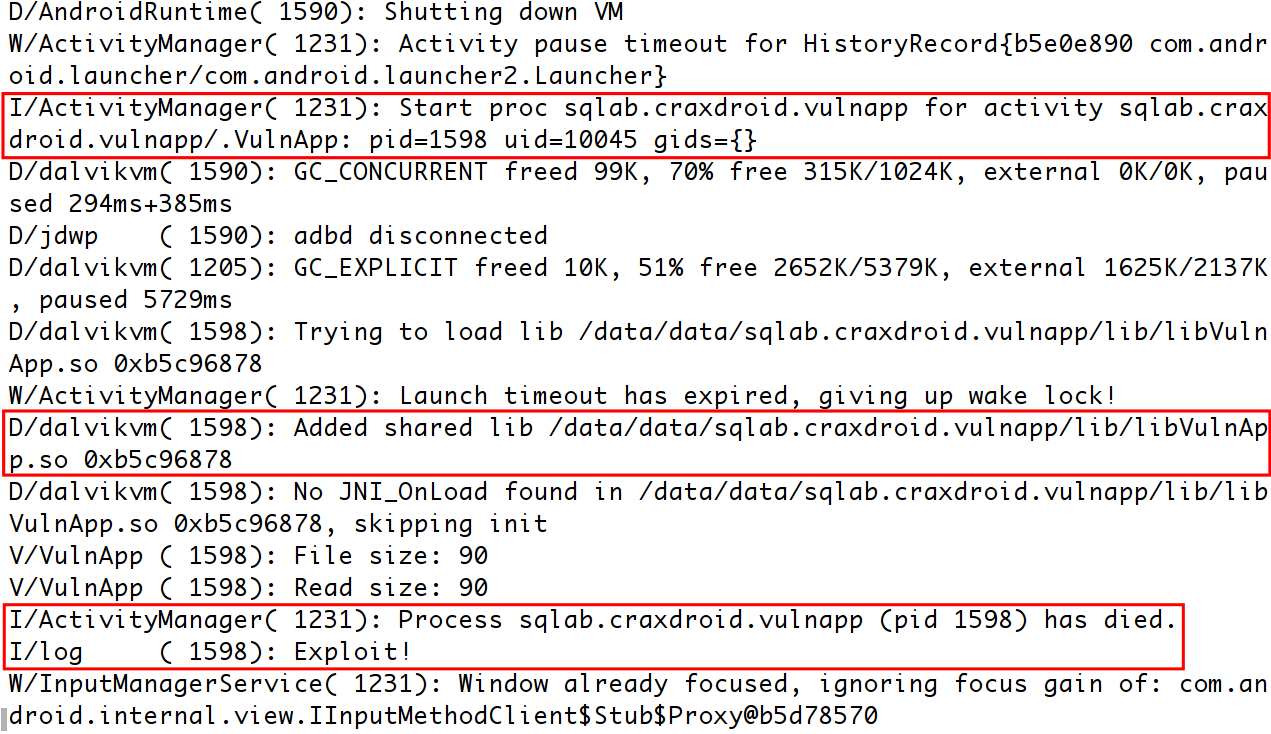
\includegraphics[width=\textwidth]{exploit-verify}
  \caption{Android x86 Exploit Verification}
  \label{fig:exploit-verify}
\end{figure}

Finally, the generated exploit file is fed back to the vulnerable app to verify
that it is a usable exploit. As shown in Figure~\ref{fig:exploit-verify}, the
vulnerable app is fired up and loads the native library correctly. The process
is then hijacked by our exploit. The ActivityManger figures out that the
process is dead, so it logs down the incident. And the following message -
``Exploit!'', indicates that the exploit succeeds.

